%******************************************************************************************
%                           Top-Level FPGALink User Manual
%******************************************************************************************

% Makestuff style and defs
% Stop LaTeX defaulting to US Letter
\documentclass[english,a4paper,12pt]{article}

% The Makefile substitutes MAKESTUFF_GEOMETRY to select parameters for print
% version or the mobile device version (Kindle, iPad, etc).
\usepackage[width=15.3cm, height=23cmMAKESTUFF_GEOMETRY]{geometry}

% Packages to use
\usepackage[colorlinks=true,linkcolor=black,urlcolor={[rgb]{0.00,0.00,0.40}},linktoc=all]{hyperref}
\usepackage{graphicx}
\usepackage[compact]{titlesec}
\usepackage{alltt}
\usepackage[font=small,labelfont=bf]{caption}
\usepackage[num]{isodate}

% Enable bold monospace
\renewcommand{\ttdefault}{txtt}

% Spacing...
\parindent=0pt
\parskip=2ex

% Settings for section headings: large, bold, centred
\titleformat{\section}[hang]{\Large\sffamily\bfseries\filcenter}{\thesection}{1em}{}

% Settings for subsection headings: smaller, bold, left-justified
\titleformat{\subsection}[hang]{\large\sffamily\bfseries}{\thesubsection}{1em}{}
\titlespacing{\subsection}{0pt}{5ex}{0ex}

% Settings for subsubsection headings: normal size but still bold
\titleformat{\subsubsection}[hang]{\sffamily\bfseries}{\thesubsubsection}{1em}{}
\titlespacing{\subsubsection}{0pt}{2ex}{0ex}

% List macro
\newenvironment{blobs}
{\begin{itemize}
  \setlength{\itemsep}{1ex}
  \setlength{\parskip}{1ex}
  \setlength{\parsep}{0pt}}
{\end{itemize}}

% Description macro
\newenvironment{desc}
{\begin{description}
  \setlength{\itemsep}{2ex}
  \setlength{\parskip}{2ex}
  \setlength{\parsep}{0pt}}
{\end{description}}

% Image macros
\newcommand{\imgcap}[2]{%
  \begin{figure}[h]%
  \centerline{\includegraphics[width=\linewidth]{images/#1}}%
  \caption{#2}%
  \end{figure}}

\newcommand{\img}[1]{%
  \centerline{\includegraphics[width=\linewidth]{images/#1}}}

% Code snippet macros
\newcommand{\codecap}[2]{%
  \begin{figure}[h]%
  {\footnotesize \input{tmp/#1}}%
  \caption{#2}%
  \end{figure}}

% Code snippet macro
\newcommand{\code}[2]{%
  {\footnotesize \input{tmp/#1}}}

% Settings for code snippets
\input{tmp/pygments}

% DocTitle macro
\newcommand{\doctitle}[4]{%
  {\Huge\sffamily\bfseries\centerline{#2}}%
  \vspace*{0.25cm}%
  {\Large\sffamily\bfseries\centerline{#3}}%
  \vspace*{0.5cm}%
  {\footnotesize\sffamily\centerline{{\copyright\the\year}{ }{#4}}}%
  \vspace*{1cm}%
  \img{#1}
  \vfill%
  \centerline{
\includegraphics[width=2cm]{images/by-sa}}%
  \vspace*{0.25cm}%
  {\scriptsize\sffamily\centerline{\href{http://creativecommons.org/licenses/by-sa/3.0/}{This work is licensed under the Creative Commons Attribution-ShareAlike 3.0 Unported License}}}%
}

% ISO date
\newcommand{\isotoday}[1]{%
  {\isodash{}\isodate\today}}

\newcommand*\justify{%
  \fontdimen2\font=0.4em% interword space
  \fontdimen3\font=0.2em% interword stretch
  \fontdimen4\font=0.1em% interword shrink
  \fontdimen7\font=0.1em% extra space
  \hyphenchar\font=`\-% allowing hyphenation
}


\begin{document}
\vspace*{2cm}
\doctitle{fpgalinkOverview}{FPGALink User Manual}{(Verilog Edition)}{Chris McClelland/MakeStuff.eu}

\newpage
\tableofcontents

\newpage
\section{Introduction}
\subsection{Justification}
Development kits for Field Programmable Gate Arrays (FPGAs) are ubiquitous, with offerings from a plethora of manufacturers, with prices ranging from the tens of dollars to well into the thousands, and featured FPGAs ranging from a few thousand logic cells to a few million. Whereas the high-end boards tend to be PCIx plug-in cards, the cheaper boards tend either to be designed around a USB interface chip (e.g Cypress FX2LP, Atmel AVR, Microchip PIC or FTDI chip), or lack direct host interfacing altogether, requiring a standalone JTAG cable for programming.

Unfortunately, even for those boards designed around a USB interface, there is a general lack of good integrated solutions for exchanging arbitrary data between the host computer and the FPGA, once it has been programmed.

\subsection{Overview}
FPGALink is an end-to-end, open-source, cross-platform solution designed to do a couple of simple jobs, and do them well:

\begin{blobs}
  \item
    Program an FPGA with JTAG, either from an onboard configuration source or over USB.
  \item
    Allow the host and/or microcontroller to exchange arbitrary binary data with the FPGA.
\end{blobs}

It provides a host-side API, firmware for several USB interface microcontrollers, and 128 addressable eight-bit read/write FIFOs on the FPGA side.

\begin{blobs}
  \item
    On the host side there is a dynamic-link library with a straightforward API. Library and example application binaries are provided for MacOSX (x64 \& x86), Windows (x64 \& x86) and Linux (x64, x86, ARM \& PowerPC). Bindings are provided for C/C++, Python and Excel/VBA, but binding other languages is straightforward.
  \item
    For the USB interface there are firmwares for the Cypress FX2LP (used on most Digilent, KNJN, ZTEX and Opal Kelly boards) and Atmel AVR (used by some AVNet and Digilent boards). Support for the FTDI chips is planned.
  \item
    The Cypress FX2LP firmware supports a synchronous FIFO interface with a sustained bandwidth of around 42MiB/s. The Atmel AVR firmware supports an asynchronous interface\footnote{Actually IEEE 1284 in Enhanced Parallel Port mode.} with a sustained bandwidth of around 1.2MiB/s. Other microcontroller-to-FPGA protocols such as SPI are planned.
  \item
    For the FPGA there is a simple interface module which when instantiated in your design gives the host a FIFO-style read/write interface, supporting up to 128 separate logical ``channels'' into your design. A couple of fully-functional example designs are provided to get you started.
\end{blobs}

Everything is licensed under the GNU Lesser General Public Licence\footnote{\url{http://www.gnu.org/copyleft/lesser.html}}; you are therefore free to distribute unmodified copies of FPGALink with your products. The library has no commercial or hardware usage restrictions, so you can prototype your design with an inexpensive devkit, and then use the same software tools on your custom-built PCBs. In this way you can easily distribute updated FPGA designs to your customers just as you would with regular firmware updates, with no special programming cables required, making your FPGA truly ``field-programmable''.

\subsection{Document Conventions}
Whilst describing interactive console sessions, I will use {\bf\textcolor[rgb]{0.00,0.00,0.00}{\texttt{monospace bold}}} for characters entered by a human and {\textcolor[rgb]{0.20,0.20,0.20}{\texttt{monospace regular}}} for the computer's responses.

Remember:
\begin{blobs}
  \item 1MB = 1 megabyte = 10\textsuperscript{6} bytes = 1,000,000 bytes.
  \item 1MiB = 1 mebibyte = 2\textsuperscript{20} bytes = 1,048,576 bytes.
  \item 1Mb = 1 megabit = 10\textsuperscript{6} bits = 1,000,000 bits.
  \item 1Mib = 1 mebibit = 2\textsuperscript{20} bits = 1,048,576 bits.
\end{blobs}

\subsection{How to Get Help}
The only place you're \textit{guaranteed} to get a response to FPGALink-related queries is the FPGALink Users Group at \url{http://groups.google.com/group/fpgalink-users}.

\newpage
\subsection{Licences \& Disclaimers}
The FPGALink library, firmware \& Verilog code is licensed under the LGPLv3\footnote{\url{http://www.gnu.org/copyleft/lesser.html}}:

\begin{quote}
Copyright \copyright 2009-{\the\year} Chris McClelland

FPGALink is free software: you can redistribute it and/or modify it under the terms of the GNU Lesser General Public License as published by the Free Software Foundation, either version 3 of the License, or (at your option) any later version.

FPGALink is distributed in the hope that it will be useful, but WITHOUT ANY WARRANTY; without even the implied warranty of MERCHANTABILITY or FITNESS FOR A PARTICULAR PURPOSE. See the GNU Lesser General Public License for more details.
\end{quote}

The FLCLI utility is licensed under the GPLv3\footnote{\url{http://www.gnu.org/copyleft/gpl.html}}:

\begin{quote}
Copyright \copyright 2009-{\the\year} Chris McClelland

FLCLI is free software: you can redistribute it and/or modify it under the terms of the GNU General Public License as published by the Free Software Foundation, either version 3 of the License, or (at your option) any later version.

FLCLI is distributed in the hope that it will be useful, but WITHOUT ANY WARRANTY; without even the implied warranty of MERCHANT-ABILITY or FITNESS FOR A PARTICULAR PURPOSE. See the GNU General Public License for more details.
\end{quote}

\newpage
\section{Getting Started}

\subsection{Installation}
First, download the FPGALink binary distribution. This manual assumes you're using the \texttt{\href{http://www.swaton.ukfsn.org/bin/fpgalink-MAKESTUFF_TODAY_DATE/fpgalink-bin.tar.gz}{fpgalink-MAKESTUFF_TODAY_DATE release}}.

\begin{desc}
  \item[\sffamily{Linux:}] \hfill \\
    Just download the binary distribution and unpack it into your home directory. Things will work out-of-the-box on most modern distributions.

    Separate sets of binaries for x64, x86, ARM and PowerPC architectures are provided in the \texttt{lin.*} directories. For ARM there are two sets of binaries: \texttt{armel} for the soft-float ABI and \texttt{armhf} for the hard-float ABI.

    To grant regular users permission to access the USB devices you'll be using, you will need to add \texttt{udev} rules. First check which groups you're in by running ``\texttt{groups}'', choose a group (I chose ``\texttt{users}'') and then for each USB device (i.e, each VID:PID), add a line to \texttt{/etc/udev/rules.d/10-local.rules}:

    \code{cli/udev}

    Ensure the VID:PID is lowercase. You may need to restart the udev service with \texttt{sudo service udev restart}, but you will definitely need to unplug and reconnect the device(s) in order to activate the new permissions.

  \item[\sffamily{Windows:}] \hfill \\
    You may need to install the VC++ 2010 redistributable package:
    \begin{blobs}
      \item
        For x86: \href{http://download.microsoft.com/download/5/B/C/5BC5DBB3-652D-4DCE-B14A-475AB85EEF6E/vcredist_x86.exe}{vcredist\_x86.exe}
      \item
        For x64:  \href{http://download.microsoft.com/download/3/2/2/3224B87F-CFA0-4E70-BDA3-3DE650EFEBA5/vcredist_x64.exe}{vcredist\_x64.exe}
    \end{blobs}
    You will need to install a USB driver for your board:
    \begin{blobs}
      \item
        Uninstall any existing drivers for your device.
      \item
        Download \href{http://sourceforge.net/projects/libwdi/files/zadig/}{Zadig}, unpack it with \href{http://www.7-zip.org/download.html}{7-Zip} and run \texttt{zadig.exe}.
      \item
        Select your device in the drop-down list.
      \item
        Select either ``libusbK'' or ``WinUSB''.
      \item
        Click ``Install Driver''.
    \end{blobs}
    Also, although it's not strictly required, all the command-line examples in this manual assume you're using the \href{http://www.makestuff.eu/wordpress/?page_id=1489}{MakeStuff Build Infrastructure}. It's also \textit{the only supported build platform on Windows}, so whilst you're free to use something else, you're on your own if you do.

    Separate sets of binaries for x64 and x86 architectures are provided in
    the \texttt{win.*} directories.
  \item[\sffamily{MacOSX:}] \hfill \\
    You just need to install \href{http://www.swaton.ukfsn.org/bin/libusbx-macosx}{libusbx-1.0.x} and you're good to go.

    One set of universal binaries for x64 and x86 architectures is provided in the \texttt{darwin} directory.
\end{desc}

\subsection{Supported Boards}
By providing multiple ``board support packages'' (BSPs), FPGALink is able to support several different FPGA development kits, based on Xilinx or Altera FPGAs and Atmel AVR or Cypress FX2LP USB microcontrollers\footnote{Porting to other boards based on these components is usually fairly trivial; if you have such a board, ask on the \href{http://groups.google.com/group/fpgalink-users}{mailing list}.}. The BSPs are implemented as a hierarchy: at the top level there are one or more \textit{templates}, which provide an abstract description of the host-FPGA connection. Each template has one or more supported \textit{boards}, each of which can be thought of as a concrete instantiation of the template for a given board: the actual FPGA device, its pinout, etc.

A pair of fully-functional examples is provided, with ready-to-go programming files for each of the supported FPGA boards. The first example is \texttt{cksum}, which we will play with in the next section, and the second is \texttt{fifo}. Both use various bits of board I/O to provide some interaction and visual feedback:

\begin{blobs}
  \item
    Eight slider-switches, providing eight bits of input data.
  \item
    Eight LEDs, providing visual feedback of an eight-bit binary value.
  \item
    Four seven-segment displays, wired with common cathodes and an anode for each digit, providing visual feedback of a sixteen-bit hexadecimal value (and an additional four-bit binary value via the four decimal point LEDs).
\end{blobs}

Obviously, not all of the supported FPGA boards include all of these I/O features, and may have other special requirements before the supplied examples will work. However, the examples are written such that it's possible to monitor their operation in a limited way through the USB connection.

\subsubsection{Cypress FX2LP-Based Boards}

The Cypress FX2LP is a Hi-Speed (480Mb/s) USB interface. It is capable of transferring data between an FPGA and the host at about 42MiB/s, using an eight-bit synchronous FIFO interface. Although fast and fairly cheap, it has a rather eccentric internal architecture, so custom firmware development is not recommended.

\begin{desc}
  \item[\sffamily{\href{http://www.digilentinc.com/Products/Detail.cfm?Prod=Nexys3}{Digilent Nexys3}:}] \hfill \\
    There are no special considerations for the Nexys3.
  \item[\sffamily{\href{http://www.digilentinc.com/Products/Detail.cfm?Prod=NEXYS2}{Digilent Nexys2 (500K \& 1200K versions)}:}] \hfill \\
    Separate BSPs are provided for the 500K and 1200K gate versions. Also, when the Nexys2 ``power select'' jumper is set to ``USB'', the FPGA is supplied with power via a little FET on the board which is under software control. Therefore before programming the FPGA it's necessary to turn this FET on.
  \item[\sffamily{\href{http://www.digilentinc.com/Products/Detail.cfm?Prod=ATLYS}{Digilent Atlys}:}] \hfill \\
    The Atlys has the requisite LEDs and switches, but does not have a display of any kind, so on Atlys the provided examples map the seven-segment display signals to the first twelve pins on the board's VHDCI connector. Unless you know exactly what you're doing, please ensure you have nothing connected to the VHDCI port before you begin.
  \item[\sffamily{\href{http://www.knjn.com/shop.html?pg=pic&src=images/Board_Xylo-L_details.jpg\&title=The\%20Xylo-L\%20board}{KNJN Xylo-L}:}] \hfill \\
    Since the Xylo-L has no onboard peripherals, the provided examples map the switches, LEDs and seven-segment displays to the board's expansion connector marked H4. Unless you know exactly what you're doing, please ensure you have nothing connected to the H4 port before you begin.
  \item[\sffamily{\href{http://www.digilentinc.com/Products/Detail.cfm?Prod=S3BOARD}{Digilent S3BOARD}:}] \hfill \\
    There is only partial support for the S3BOARD, because it does not include a USB interface of any kind; instead, it is supplied with a parallel-port JTAG cable. To use the S3BOARD with FPGALink, you will need an external FX2LP board with the appropriate connections\footnote{\href{http://www.makestuff.eu/wordpress/electronics/fx2fpga/}{FX2FPGA} serves as a reference design, but suitable commercial boards are also available.}.
  \item[\sffamily{\href{http://www.makestuff.eu/wordpress/electronics/lx9-fpga-board}{MakeStuff LX9}:}] \hfill \\
    The MakeStuff LX9 is intended to be a cheap, home-solderable, repurposable FPGA board incorporating a Xilinx XC6SLX9 FPGA, FX2LP, SDRAM, SD-card slot and 47 (or 51 if the SD-card slot is not needed) well-grounded FPGA I/Os.
\end{desc}

\subsubsection{Atmel AVR-Based Boards}

The USB-capable Atmel AVR8 microcontrollers (AT90USB* \& ATMEGA*U*) are very cheap, and they incorporate a Full-Speed (12Mb/s) USB interface. They are capable of transferring data between an FPGA and the host at between 330KiB/s and about 1.2MiB/s, using an eight-bit asynchronous EPP-style interface. Although slower than the FX2LP, they are much more popular as general-purpose microcontrollers, and much easier to program, making custom firmware development fairly straightforward.

\begin{desc}
  \item[\sffamily{Minimus/EP2C5 Board:}] \hfill \\
    You can buy\footnote{e.g from \href{http://www.modtraders.co.uk/minimus-32-avr-usb-development-board.html}{ModTraders} and \href{www.ebay.co.uk/itm/150835820710}{eBay}, respectively} a Minimus ATMEGA32U2 board for \textsterling{}6, and an EP2C5 Mini Board for \textsterling{}13. With suitable interconnects, the pair make up by far the cheapest FPGALink-capable hardware solution.
  \item[\sffamily{Minimus/Nexys2 Board:}] \hfill \\
    There is also a BSP for a Minimus board attached to a Nexys2-1200. It is unlikely to be of interest because the Nexys2-1200 already has a superior FX2LP-based USB interface.
\end{desc}

Both of these boards require custom wiring, which is described in \hyperref[apdx:custom]{Appendix~\ref*{apdx:custom}}.

\newpage
\subsection{The \texttt{flcli} Utility}
Since FPGALink is a library, you would normally just embed it into your application, but in order to get you started, the FPGALink binary distribution includes \texttt{flcli}\footnote{Unlike the rest of FPGALink, the \texttt{flcli} utility is licensed under the terms of the GNU General Public License. See \url{http://www.gnu.org/copyleft/gpl.html}}, a small command-line utility which provides access to some of the library's features.

\code{cli/flcli_help}

\begin{desc}
  \item[\texttt{--ivp=<VID:PID> [FX2LP-specific]}] \hfill \\
    The FX2LP microcontroller has no onchip nonvolatile storage, so it loads its firmware from an external EEPROM and/or has its firmware loaded over USB. The \texttt{flcli} utility first tries to connect to the device specified by \texttt{--vp}; if it fails, it tries to load firmware into the device specified by \texttt{--ivp}.
  \item[\texttt{--jtag=<portSpec> [FX2LP-specific]}] \hfill \\
    By default the FX2LP firmware's JTAG interface is compatible with the wiring on Digilent boards (\texttt{TDO}, \texttt{TDI}, \texttt{TMS} \& \texttt{TCK} connected to port D bits 0, 2, 3 \& 4 respectively.) If your board has different connections, you will need to specify which port lines to use along with \texttt{--ivp}. The port specification is the port (``A'', ``C'' or ``D'') followed by four digits for the port bits to use for \texttt{TDO}, \texttt{TDI}, \texttt{TMS} \& \texttt{TCK}. For example, the Xylo-L board uses a JTAG port of ``\texttt{D1240}'' and the MakeStuff LX9 uses ``\texttt{A7031}''. Only bits 0, 1, 3 \& 7 are available for JTAG on port A.
  \item[\texttt{--vp=<VID:PID>}] \hfill \\
    The FPGALink device to connect. This may either be a regular \texttt{<VID:PID>} (e.g \texttt{1D50:602B}) or it may include an additional device ID (e.g \texttt{1D50:602B:0006}). The device ID may be used to distinguish between multiple FPGALink devices sharing the same \texttt{<VID:PID>}.
  \item[\texttt{--digport=<S:MM:DD:PP}] \hfill \\
    Configure general-purpose port pins and data directions.
  \item[\texttt{--query}] \hfill \\
    Print an IDCODE for each device in the JTAG chain.
  \item[\texttt{--xsvf}] \hfill \\
    Play the specified \texttt{.svf}, \texttt{.xsvf} or \texttt{.csvf} file into the JTAG chain. This is typically (but not necessarily) used for FPGA programming.
  \item[\texttt{--action=<actionString>}] \hfill \\
    Execute the semicolon-separated list of CommFPGA commands, for reading and writing FPGA channels.
  \item[\texttt{--cli}] \hfill \\
    Start a command-line interface for executing CommFPGA commands.
  \item[\texttt{--benchmark}] \hfill \\
    Output a measured throughput (in MiB/s) and 16-bit checksum for each transfer.
\end{desc}

The \texttt{--cli} and \texttt{--action=<actionString>} options support three commands, ``\texttt{r}'' (read), ``\texttt{w}'' (write) and ``\texttt{q}'' (quit). The syntax of the read command is as follows:

\begin{quote}
\textbf{\texttt{r<channel> [<count> [<fileName>]]}}

\begin{desc}
  \item[\texttt{channel:}] \hfill \\
    The FPGA channel, 0-7F.
  \item[\texttt{count:}] \hfill \\
    How many bytes (in hex) to read from the FPGA channel, default 1.
  \item[\texttt{fileName:}] \hfill \\
    A binary file (in single or double-quotes) to write the FPGA's data to.
\end{desc}
\end{quote}

If you don't specify a \texttt{fileName}, the FPGA's data is printed to stdout as a hex dump.

\newpage
The syntax of the write command is as follows:

\begin{quote}
\textbf{\texttt{w<channel> <byteSeq | fileName>}}

\begin{desc}
  \item[\texttt{channel:}] \hfill \\
    The FPGA channel, 0-7F.
  \item[\texttt{byteSeq:}] \hfill \\
    A sequence of hex bytes to be written to the FPGA channel,\\e.g \texttt{0123456789abcdef}.
  \item[\texttt{fileName:}] \hfill \\
    An existing binary file (in single or double-quotes) to dump into the FPGA.
\end{desc}
\end{quote}

All numbers are in hexadecimal. Since a byte is two hex digits, the \texttt{byteSeq} must have an \textit{even} number of digits. Filenames must be quoted using single-quotes(\texttt{'}) or double-quotes (\texttt{"}). You may put several read and/or write commands on one line, separated by semicolons (\texttt{;}).

For example, \texttt{w1 00;w2 00;w0 "datafile.dat";r1;r2} first writes \texttt{0x00} to channels 1 \& 2, then writes the contents of \texttt{datafile.dat} to channel 0, and finally reads one byte from channels 1 \& 2.

\newpage
\subsection{Programming the FPGA}
Using the \texttt{flcli} utility, we can now program the FPGA for the first time. Programming is done by playing a scripted set of JTAG operations into the FPGA's JTAG port.

\img{jtag}

You can program the FPGA like this:

\code{cli/prog_cksum_verilog}

You will need to replace \texttt{<PLATFORM>}, \texttt{<VID:PID>}, \texttt{<JTAG>}, \texttt{<TEMPLATE>} and \texttt{<BOARD>} in the above command-line with values appropriate for your specific host platform and FPGA board:

\begin{desc}
  \item[\texttt{<PLATFORM>}] \hfill \\
    Your host platform. This will be one of \texttt{win.x64}, \texttt{win.x86}, \texttt{osx}, \texttt{lin.x64}, \texttt{lin.x86}, \texttt{lin.armhf}, \texttt{lin.armel} or \texttt{lin.ppc}.
  \item[\texttt{<VID:PID>}] \hfill \\
    The correct vendor and product IDs for your board. For \texttt{-i} this will be:
    \begin{blobs}
      \item \texttt{1443:0005} for Nexys2
      \item \texttt{1443:0007} for Nexys3 \& Atlys
      \item \texttt{04B4:8613} for Xylo-L \& MakeStuff LX9
    \end{blobs}
    You can either set \texttt{-v} to the same as \texttt{-i}, or you can use the official FPGALink \texttt{<VID:PID>} of \texttt{1D50:602B}. If you have multiple FPGALink devices you can assign a different device ID to each, e.g ``\texttt{-v 1D50:602B:0002}'', ``\texttt{-v 1D50:602B:0003}'', etc.
  \item[\texttt{<JTAG>}] \hfill \\
    The correct FX2LP port connections for the FPGA's four JTAG pins TDO, TDI, TMS \& TCK. This will be:
    \begin{blobs}
      \item \texttt{D0234} for Digilent boards
      \item \texttt{D1240} for Xylo-L
      \item \texttt{A7031} for MakeStuff LX9
    \end{blobs}
  \item[\texttt{<TEMPLATE>}] \hfill \\
    An identifier for how your board wires its FPGA to the outside world. This will be \texttt{fx2min}, \texttt{fx2all} or \texttt{epp}.
  \item[\texttt{<BOARD>}] \hfill \\
    The name of your board, which will be one of \texttt{nexys2-500}, \texttt{nexys2-1200}, \texttt{nexys3}, \texttt{atlys}, \texttt{xylo-l}, \texttt{s3board}, \texttt{ep2c5} or \texttt{lx9}.
\end{desc}

There are some caveats:

\begin{desc}
  \item[\sffamily{Nexys2 Users:}] \hfill \\
    If your board's ``power select'' jumper is set to ``USB'', it will be necessary to switch on the FPGA's power by supplying an additional \texttt{-p} command-line option.
  \item[\sffamily{AVR-Based Boards:}] \hfill \\
    The \texttt{-i <VID:PID>} and \texttt{-j <JTAG>} options are only needed for FX2LP-based boards. It is not needed for AVR-based boards because these parameters are set at AVR firmware compile-time.
\end{desc}

If successful, you should see the ``Done'' light on your board switch on, and ``\texttt{0000}'' appear on your board's seven-segment display. If your board does not have either of these, don't worry; as long as the \texttt{flcli} command completed without error, you can proceed to the next section.

So what just happened? Well, \texttt{flcli} loaded new firmware if necessary (FX2LP-based boards only), then powered up the FPGA (Nexys2 only), then scanned the board's JTAG chain for attached devices, and finally loaded a pre-built design file for the \texttt{cksum} example into the FPGA.

In this case we used a \texttt{.csvf} file\footnote{The CSVF format is similar to Xilinx's XSVF, but it's better suited for playback by small microcontrollers, and is much more space-efficient.} to program the FPGA, but FPGALink directly supports the \texttt{.svf} files generated by the Xilinx and Altera tools, as well as the Xilinx-specific \texttt{.xsvf} format.

\subsection{Interacting with the FPGA (Part 1)}
A couple of interface modules are supplied, ``\texttt{comm\_fpga\_fx2}''\footnote{\texttt{hdl/libs/makestuff/comm\_fpga/fx2/verilog/comm\_fpga\_fx2.v}.} and ``\texttt{comm\_fpga\_epp}''\footnote{\texttt{hdl/libs/makestuff/comm\_fpga/epp/verilog/comm\_fpga\_epp.v}.} for you to instantiate in your application's Verilog code. The former has an external interface compatible with the Cypress FX2LP's slave FIFO signals and the latter has an external interface compatible with the EPP signals provided by the Atmel AVR firmware. However, both have identical \textit{internal} interfaces, each providing a read pipe, a write pipe and a seven-bit address specifying which of 128 logical \textit{channels} is to be read or written.

\img{comm}

Each channel is eight bits wide. Each channel may be read from or written to by the host. Each read or write operation can deal with single bytes or many hundreds of megabytes. Applications are free to choose how these channels are implemented in their Verilog code. Two such implementations are given in the \texttt{cksum} and \texttt{fifo} examples.

In the previous section, we loaded the \texttt{cksum} example into the FPGA. The \texttt{cksum} example implements the FPGA channels using ordinary registers, meaning that a write to channel N merely updates register N inside the FPGA, and a read from channel N typically returns the current value of register N.

You can see this by using \texttt{flcli}'s command-line mode (triggered by the \texttt{-c} option):

\code{cli/comm_cksum}

The instructions accepted by the command-line are terse, but simple.

The ``\texttt{w1 00;w2 00;w0 cafebabef00d1e;r1;r2;r0 4}'' command line performs six operations sequentially:

\begin{blobs}
  \item Write single byte \texttt{0x00} to channel 1.
  \item Write single byte \texttt{0x00} to channel 2.
  \item Write \textbf{seven} bytes \texttt{0xCA}, \texttt{0xFE}, \texttt{0xBA}, \texttt{0xBE}, \texttt{0xF0}, \texttt{0x0D}, \texttt{0x1E} to channel 0.
  \item Read one byte \texttt{0x04} from channel 1.
  \item Read one byte \texttt{0x2B} from channel 2.
  \item Read \textbf{four} bytes from channel 0.
\end{blobs}

The \texttt{cksum} example maintains a running 16-bit checksum of the bytes written to channel 0; the checksum itself is available on channels 1 \& 2. Notice that the checksum value read from channels 1 \& 2 is \texttt{0x045B}, which is the same as the checksum value reported by \texttt{flcli} for the seven-byte transfer: the checksum calculated by \texttt{flcli} matches the checksum calculated by the FPGA. The four reads from channel 0 just return the state of the eight switches on the board.

The ``\texttt{w1 ca;w2 fe;r1;r2}'' command line performs four operations sequentially:

\begin{blobs}
  \item Write single byte \texttt{0xCA} to channel 1.
  \item Write single byte \texttt{0xFE} to channel 2.
  \item Read one byte \texttt{0xCA} from channel 1.
  \item Read one byte \texttt{0xFE} from channel 2.
\end{blobs}

Channels 1 \& 2 are implemented as the MSB \& LSB of the 16-bit checksum register, so values written may be read back.

You can see how this is implemented in the FPGA by taking a look at the Verilog\footnote{See \texttt{hdl/apps/makestuff/swled/cksum/verilog/cksum\_rtl.v} for the complete module.}:

\code{verilog/registers}

So ``\texttt{w1 ca}'' writes a single byte to channel 1, which sets \texttt{chanAddr\_in=0x01} and \texttt{h2fData\_in=0xCA}, and drives \texttt{h2fValid\_in} high for one clock cycle, which writes the value \texttt{0xCA} to the LSB of the checksum register (preserving the MSB).

Similarly when you enter ``\texttt{r2}'', it initiates a single byte read of channel 2, which sets \texttt{chanAddr\_in=0x02} and drives \texttt{f2hReady\_in}\footnote{Actually, since the value stored in a simple register like this is unaffected by a read operation, it's not necessary for this code to consider \texttt{f2hReady\_in} - it need only select the correct register value with which to drive \texttt{f2hData\_out}, and do so continuously.} high for one clock cycle, causing the MSB of the checksum register to be sampled and returned to the host.

Channel 0 is a little more interesting. Bytes written (e.g ``\texttt{w0 aa}'') are displayed on the eight board LEDs and also added to the running sixteen-bit checksum shown on the seven-segment display. Conversely, reads return the current state of the eight switches.

Notice that reads and writes never block: there is always data available in the read pipe and there is always room available in the write pipe.

\subsection{Interacting with the FPGA (Part 2)}
In the previous section, we used the \texttt{flcli} utility to read and write simple registers implemented in the FPGA by the \texttt{cksum} example. The \texttt{fifo} example is more interesting. You can load it like this:

\code{cli/prog_fifo_verilog}

Now, channel 0 is connected to a pair of FIFOs inside the FPGA, a read FIFO and a write FIFO. Independent producer and consumer processes periodically insert upcount data into the read FIFO and drain data from the write FIFO, respectively. The speed at which these processes work is selectable by setting different values on the eight switches: \texttt{sw[7:4]} controls the speed of the consumer and \texttt{sw[3:0]} controls the speed of the producer.

Here's the code\footnote{See \texttt{hdl/apps/makestuff/swled/fifo/verilog/fifo\_rtl.v} for the complete module.}:

\code{verilog/fifos}

When the host writes to channel 0, each byte is clocked into the write FIFO. When the write FIFO fills up, \texttt{h2fReady\_out} is deasserted which tells the host to stop sending until the consumer process has freed up some room for more data.

When the host reads from channel 0, each byte is clocked out of the read FIFO. When the read FIFO empties, \texttt{f2hValid\_out} is deasserted to stop sending data to the host until the producer process has inserted some more data into the FIFO.

When the example is first loaded, you will see the leftmost pair of digits on the seven-segment display incrementing, telling you how many bytes there are in the read FIFO. When you issue the command \texttt{r0 10}, the host reads sixteen bytes from the read FIFO, causing the count to decrement by sixteen. If there are as yet insufficient bytes in the read FIFO to fulfill the request, the host blocks until bytes become available.

Similarly, the rightmost pair of digits on the seven-segment display tells you how many bytes there are in the write FIFO. When you issue the command \texttt{w0 010204081020408 04020100804020100}, sixteen bytes are written to the write FIFO. The consumer process then begins to drain the data, displaying each byte in turn on the eight LEDs. If there is as yet insufficient room in the write FIFO to fulfill the request, the host blocks until enough room is available. This is not always noticeable because the microcontrollers have additional bytes of FIFO space.

If your board does not have a seven-segment display, you can read the current depth of the write FIFO by reading from channel 1, and you can read the current depth of the read FIFO by reading from channel 2.

\subsection{Summary}
In this chapter we used the \texttt{flcli} utility to program an FPGA with a couple of pre-built examples, and to communicate with the data channels in the FPGA.

\newpage
\section{Host Application Development}
The \texttt{flcli} utility is a great way to get started with FPGALink, and for simple testing of the behaviour of your Verilog code, but sooner or later you will want to dive in and write your own host-side applications. There is out-of-the-box support for C/C++, Python and Excel/VBA, but the core library itself is just a C DLL, so calling into it from other languages is straightforward\footnote{Or at least it \textit{ought} to be straightforward!}.

In order to enable an application to communicate with potentially many FPGALink devices, the library uses the concept of a ``handle'' to refer to an FPGALink device. An opaque handle is returned when a connection is first established to a device, and that handle is supplied for all subsequent operations on that device.

\subsection{Language Bindings}
There is obviously a significant cross-language semantic overlap in the API; the only differences are those imposed by the languages themselves.

\subsubsection{C}
Because C has no concept of exceptions, wherever a function \textit{can} fail, its return value is just a status code; the actual result (if any) is provided in an ``out'' parameter instead. An optional error message is also provided in an ``out'' parameter. Conversely, wherever a function \textit{cannot} fail, its return value (if any) is actually the result.

Each function that \textit{can} fail will return \texttt{FL\_SUCCESS} on success, or something else on failure. Each will also accept a pointer to a \texttt{const char*} which will be set to a more or less meaningful message if an error occurs. The memory for this message is dynamically allocated and must subsequently be deallocated by application code with \texttt{flFreeError()}. If you do not wish to receive error messages you can just set this parameter to \texttt{NULL}.

It's useful to define a macro to handle this:

\code{c/check_macro}

To get you started, there is an example in C for you to study in the \texttt{examples/c} subdirectory. See \texttt{examples/c/README} for details of how to compile the code on your platform.

\subsubsection{Python}
Python has exceptions, so the API in Python is written such that each function's return value (if any) is actually its result, with an exception thrown when an error occurs.

Separate bindings are provided for Python2.x and Python3.x. These reside in the \texttt{examples/python} subdirectory. The bindings are themselves executable, and offer similar functionality to the C example. The Python binding may be imported into your own code, or used from an interactive Python session. For more details, see \texttt{examples/python/README}.

\subsubsection{Excel/VBA}
VBA has exceptions, so the API in VBA is written such that each function's return value (if any) is actually its result, with an exception thrown when an error occurs.

The \texttt{examples/excel/fpgalink.xls} spreadsheet incorporates the VBA binding, and exposes a simple graphical user interface. Before opening it, please ensure you have unpacked the FPGALink distribution to a \textit{local} drive, not a network drive, otherwise Excel will consider the FPGALink DLL to be untrusted and will refuse to load it.

\subsection{API Overview}
See \url{http://www.swaton.ukfsn.org/apidocs/libfpgalink\_8h.html} for more detailed API documentation.

The library consists of five classes of functions:

\begin{blobs}
  \item Firmware operations (FX2LP-specific)
  \item Connection lifecycle operations
  \item NeroJTAG operations (programming the FPGA)
  \item CommFPGA operations (interacting with the FPGA)
  \item Miscellaneous operations
\end{blobs}

Each will now be covered in turn; please refer also to the detailed API docs.

\newpage
\subsubsection{Firmware Operations [FX2LP-Specific]}
The Cypress FX2LP USB interface has no internal nonvolatile storage for firmware. On startup it typically loads firmware from an external serial EEPROM, which is probably how your board works. You can easily load new firmware over USB, or write your new firmware to the external EEPROM using these operations.

\begin{desc}
  \item[\texttt{\href{http://www.swaton.ukfsn.org/bin/fpgalink-MAKESTUFF_TODAY_DATE/api/libfpgalink\_8h.html\#a45c33041d9f6331e378ca6092646b399}{flLoadStandardFirmware()}:}] \hfill \\
    Load standard FPGALink firmware into the FX2's RAM. 
  \item[\texttt{\href{http://www.swaton.ukfsn.org/bin/fpgalink-MAKESTUFF_TODAY_DATE/api/libfpgalink\_8h.html\#a2b134bdad721202aade02cf3e6ac675b}{flFlashStandardFirmware()}:}] \hfill \\
    Flash standard FPGALink firmware into the FX2's EEPROM, optionally appending an SVF, XSVF or CSVF initialisation stream and an FPGA initialisation stream. 
  \item[\texttt{\href{http://www.swaton.ukfsn.org/bin/fpgalink-MAKESTUFF_TODAY_DATE/api/libfpgalink\_8h.html\#ae14ca5ab58b526815c80ca09793e5e34}{flLoadCustomFirmware()}:}] \hfill \\
    Load custom firmware from a \texttt{.hex} file into the FX2's RAM.
  \item[\texttt{\href{http://www.swaton.ukfsn.org/bin/fpgalink-MAKESTUFF_TODAY_DATE/api/libfpgalink\_8h.html\#a3f39c11daf31e2c1d82b35e88ad9c804}{flFlashCustomFirmware()}:}] \hfill \\
    Flash a custom firmware from a \texttt{.hex} or \texttt{.iic} file into the FX2's EEPROM.
  \item[\texttt{\href{http://www.swaton.ukfsn.org/bin/fpgalink-MAKESTUFF_TODAY_DATE/api/libfpgalink\_8h.html\#addfaedd80f0f40c9a1f134766235b23b}{flSaveFirmware()}:}] \hfill \\
    Save existing EEPROM data to an \texttt{.iic} file.
\end{desc}

\subsubsection{Connection Lifecycle Operations}
These two operations enable you to actually establish a connection to an FPGALink device over USB.

\begin{desc}
  \item[\texttt{\href{http://www.swaton.ukfsn.org/bin/fpgalink-MAKESTUFF_TODAY_DATE/api/libfpgalink\_8h.html\#a241ac59f7ba96caba2e1262ffd0d4424}{flOpen()}:}] \hfill \\
    Open a connection to the FPGALink device at the specified VID \& PID.
  \item[\texttt{\href{http://www.swaton.ukfsn.org/bin/fpgalink-MAKESTUFF_TODAY_DATE/api/libfpgalink\_8h.html\#aec8a71aea72766e3c57fa857c5f5f742}{flClose()}:}] \hfill \\
    Close the connection to the FPGALink device.
\end{desc}

\newpage
\subsubsection{Device Capabilities and Status Operations}
These operations enable you to query the FPGALink device to find out what features it supports. Currently there are only two features: \textbf{NeroJTAG} for JTAG-programming, and \textbf{CommFPGA}, for communicating with an already-programmed FPGA.

\begin{desc}
  \item[\texttt{\href{http://www.swaton.ukfsn.org/bin/fpgalink-MAKESTUFF_TODAY_DATE/api/libfpgalink\_8h.html\#a223dc9f94043ac92e744b5b3390a3f0c}{flIsDeviceAvailable()}:}] \hfill \\
    Check if a given device is actually connected to the system.
  \item[\texttt{\href{http://www.swaton.ukfsn.org/bin/fpgalink-MAKESTUFF_TODAY_DATE/api/libfpgalink\_8h.html\#a7af1b24a52d15edd73ad19a5e392abd2}{flIsNeroCapable()}:}] \hfill \\
    Check to see if the device supports NeroJTAG.
  \item[\texttt{\href{http://www.swaton.ukfsn.org/bin/fpgalink-MAKESTUFF_TODAY_DATE/api/libfpgalink\_8h.html\#ae9c77acac33d48758fb0bfdee0c7a8d8}{flIsCommCapable()}:}] \hfill \\
    Check to see if the device supports CommFPGA.
\end{desc}

\subsubsection{NeroJTAG Operations}
The NeroJTAG operations enable you to examine the JTAG chain and program devices in the chain.

\begin{desc}
  \item[\texttt{\href{http://www.swaton.ukfsn.org/bin/fpgalink-MAKESTUFF_TODAY_DATE/api/libfpgalink\_8h.html\#a32d14b999b8e9d0befde895d4272e4ef}{flScanChain()}:}] \hfill \\
    Scan the JTAG chain and return an array of IDCODEs.
  \item[\texttt{\href{http://www.swaton.ukfsn.org/bin/fpgalink-MAKESTUFF_TODAY_DATE/api/libfpgalink\_8h.html\#ab51ec323f4cc1d81dbf2ce32c53b3b37}{flPlayXSVF()}:}] \hfill \\
    Play an SVF, XSVF or CSVF file into the JTAG chain.
\end{desc}

\subsubsection{CommFPGA Operations}
The CommFPGA operations enable you to read from and write to up to 128 logical ``channels'' implemented in the FPGA.

\begin{desc}
  \item[\texttt{\href{http://www.swaton.ukfsn.org/bin/fpgalink-MAKESTUFF_TODAY_DATE/api/libfpgalink\_8h.html\#ae9a64e022ac9607d71d9b7de80508b12}{flIsFPGARunning()}:}] \hfill \\
    Check to see whether or not the FPGA has been programmed.
  \item[\texttt{\href{http://www.swaton.ukfsn.org/bin/fpgalink-MAKESTUFF_TODAY_DATE/api/libfpgalink\_8h.html\#a0478f3526c4cdaadb844288b7e60e949}{flReadChannel()}:}] \hfill \\
    Read bytes from the specified channel into the supplied buffer.
  \item[\texttt{\href{http://www.swaton.ukfsn.org/bin/fpgalink-MAKESTUFF_TODAY_DATE/api/libfpgalink\_8h.html\#ac2b8dfb0a19a357a28af9986e6a50966}{flWriteChannel()}:}] \hfill \\
    Write bytes from the the supplied read-only buffer to the specified channel.
  \item[\texttt{\href{http://www.swaton.ukfsn.org/bin/fpgalink-MAKESTUFF_TODAY_DATE/api/libfpgalink\_8h.html\#a92ca0a05d4c363a3e9444e1b9dc9b8fa}{flAppendWriteChannelCommand()}:}] \hfill \\
    Append a write command to the end of the write buffer.
  \item[\texttt{\href{http://www.swaton.ukfsn.org/bin/fpgalink-MAKESTUFF_TODAY_DATE/api/libfpgalink\_8h.html\#a0cbf4cd4df8c8cee73a70022b3467499}{flPlayWriteBuffer()}:}] \hfill \\
    Play the write buffer into the FPGALink device immediately.
  \item[\texttt{\href{http://www.swaton.ukfsn.org/bin/fpgalink-MAKESTUFF_TODAY_DATE/api/libfpgalink\_8h.html\#a36644c7d3ec966f4983dd8d17a9b2dc4}{flCleanWriteBuffer()}:}] \hfill \\
    Clean the write buffer (if any).
\end{desc}

\subsubsection{Miscellaneous Operations}
Some operations are useful or just necessary, but don't fit into the other four categories: 

\begin{desc}
  \item[\texttt{\href{http://www.swaton.ukfsn.org/bin/fpgalink-MAKESTUFF_TODAY_DATE/api/libfpgalink\_8h.html\#a973de7f601138a3e3bb8f6e184ee9be8}{flInitialise()}:}] \hfill \\
    Initialise the library. You must call this before any of the other functions.
  \item[\texttt{\href{http://www.swaton.ukfsn.org/bin/fpgalink-MAKESTUFF_TODAY_DATE/api/libfpgalink\_8h.html\#a313f24c559a56d12518cb1e7eacdf01b}{flFreeError()}:}] \hfill \\
    Free an error allocated when one of the other functions fails.
  \item[\texttt{\href{http://www.swaton.ukfsn.org/bin/fpgalink-MAKESTUFF_TODAY_DATE/api/libfpgalink\_8h.html\#a58a48f47195b55d4921659a74d9eed5d}{flSleep()}:}] \hfill \\
    Sleep for the specified number of milliseconds.
  \item[\texttt{\href{http://www.swaton.ukfsn.org/bin/fpgalink-MAKESTUFF_TODAY_DATE/api/libfpgalink\_8h.html\#ad2fd61ccae8632d5fa180d0c468257fb}{flLoadFile()}:}] \hfill \\
    Return a newly-allocated buffer with the specified binary file loaded into it.
  \item[\texttt{\href{http://www.swaton.ukfsn.org/bin/fpgalink-MAKESTUFF_TODAY_DATE/api/libfpgalink\_8h.html\#a17909597ec81d8610c791a1ebf5f1400}{flFreeFile()}:}] \hfill \\
    Free a buffer previously returned by \texttt{flLoadFile()}.
  \item[\texttt{\href{http://www.swaton.ukfsn.org/bin/fpgalink-MAKESTUFF_TODAY_DATE/api/libfpgalink\_8h.html\#ac7c58e9d3084a9367498b9576fca2805}{flPortAccess()}:}] \hfill \\
    Access port lines on the USB interface microcontroller.
\end{desc}

\newpage
\section{FPGA Application Development}
Whilst it's possible to write your own FPGA-side code, the FPGALink distribution includes some useful tools and Verilog modules to simplify this task.

\subsection{FX2LP-Based Designs}
The most common data-transfer approach taken by the supported boards is to connect 17 FPGA I/O pins to the slave FIFO interface of a Cypress FX2LP microcontroller. This configuration is supported by instantiating the \texttt{comm\_fpga\_fx2}\footnote{See \texttt{hdl/libs/makestuff/comm\_fpga/fx2/verilog/comm\_fpga\_fx2.v}.} module, and wiring\footnote{See \texttt{hdl/apps/makestuff/swled/templates/fx2all/verilog/top\_level.v}} it up like this:

\img{fx2allHarness}

Notice that there's a top-level structural module (imaginatively called \texttt{top\_level}), which instantiates a \texttt{comm\_fpga\_fx2} infrastructure module and an ``application'' module (in this case called \texttt{swled}, for ``switches and LEDs''). Notice that:
\begin{blobs}
  \item \texttt{top\_level} instantiates \texttt{comm\_fpga\_fx2} and \texttt{swled}, and wires them together.
  \item \texttt{comm\_fpga\_fx2} knows nothing about the application's connections to the outside world.
  \item \texttt{swled} knows nothing of the details of how the USB interface works: they communicate using a well-defined contract (labelled ``DVR Pipe'').
\end{blobs}

If you're designing your own PCB, a more optimal approach is to connect the FX2LP's \texttt{FIFOADR[0]} to ground and wire \texttt{/SLRD} and \texttt{/SLOE} together \textit{outside} the FPGA (i.e on the PCB) rather than \textit{inside}, in the \texttt{top\_level} module\footnote{See \texttt{hdl/apps/makestuff/swled/templates/fx2min/verilog/top\_level.v}}, thus saving two precious FPGA I/Os:

\img{fx2minHarness}

This is the approach taken by the \href{http://www.makestuff.eu/wordpress/electronics/lx9-fpga-board}{MakeStuff LX9} board. Notice that the \texttt{comm\_fpga\_fx2} and \texttt{swled} modules are identical to those we used previously. The only changes are in the PCB layout (only 15 FX2LP-FPGA signals as opposed to 17), and in the \texttt{top\_level} structural module.

\subsection{EPP-Based Designs}
The Atmel AVR firmware implements the IEEE 1284 Enhanced Parallel Port
protocol\footnote{See \url{http://www.fapo.com/eppmode.htm}}. This is implemented using \texttt{comm\_fpga\_epp}\footnote{See \texttt{hdl/libs/makestuff/comm\_fpga/fx2/verilog/comm\_fpga\_epp.v}.}, wired\footnote{See \texttt{hdl/apps/makestuff/swled/templates/epp/verilog/top\_level.v}} like this:

\img{eppHarness}

It uses fewer signals than the FX2LP's synchronous FIFO interface, but it's also significantly slower. Since EPP is an asynchronous protocol, its signals are not synchronous to any particular clock, so the FPGA needs an arbitrary clock source for its own operation.

The EPP protocol is not as efficient as the synchronous FIFO interface of the FX2LP, but in any case the overall throughput of a system based on an Atmel AVR is limited by the USB interface and not the EPP interface. This is because unlike the Hi-Speed 480Mb/s FX2LP, the AVRs are Full-Speed 12Mb/s devices. Observed throughput is about 330KiB/s for the AVR firmware running single-buffered on an AT90USB162, ATMEGA16U2, ATMEGA32U2 or similar, and about 1.2MiB/s for the firmware running double-buffered on an AT90USB647, ATMEGA32U4 or similar.

Notice that the \texttt{swled} module is identical to the one in the two FX2LP configurations shown previously. Now, not only has the PCB layout and \texttt{top\_level} module changed, but the \texttt{comm\_fpga\_fx2} module has been replaced with \texttt{comm\_fpga\_epp}.

\subsection{Data-Valid-Ready Pipes}
Notice that the two FX2LP configurations and the EPP configuration all use exactly the same application module, \texttt{swled}. This is possible because the \texttt{comm\_fpga\_*} modules all have the same \textit{internal} interface, even if their \textit{external} interfaces differ markedly. In this way, it's possible to write application Verilog which can be made to run on a variety of different FPGA boards, even though they have entirely different designs.

\img{commFpgaAppInterface}

This common internal interface is implemented using separate host-to-FPGA and FPGA-to-host pipes, each of which follow the common data-valid-ready naming convention\footnote{See                                   
\url{http://inst.eecs.berkeley.edu/~cs150/Documents/Interfaces.pdf}} for FIFOs, plus a seven-bit channel address, which tells the application module which channel is being read from or written to.

The \texttt{h2f*} pipe carries data from the host to the FPGA, and the \texttt{f2h*} pipe carries data in the opposite direction, from the FPGA back to the host. Each pipe has three signals, \texttt{*Data} and \texttt{*Valid} which are driven by the sender, and \texttt{*Ready} which is driven by the receiver. The sender drives \texttt{*Valid} high in order to tell the receiver there's valid data on \texttt{*Data}, and the receiver can drive \texttt{*Ready} low in order to tell the sender that it's not ready to accept the data yet. The data on \texttt{*Data} is transferred from the sender to the receiver if and only if both \texttt{*Valid} and \texttt{*Ready} are high on the rising edge of the clock.

In practice, the \texttt{swled} application could be either \texttt{cksum} or \texttt{fifo}, discussed in sections 2.5 and 2.6 respectively. Obviously it's not typical for two different FPGA applications to have exactly the same interface to the outside world (i.e \texttt{swled}); in this case the two different examples were contrived to share the same interface for illustrative purposes.

\subsection{Build Infrastructure}
In the \texttt{hdl} directory is a build infrastructure capable of synthesising Verilog code into SVF files suitable for loading into an FPGA with FPGALink. Xilinx and Altera FPGA toolchains are supported. The build infrastructure uses command-line tools rather than the vendors' Integrated Development Environments, but if you prefer to work in an IDE, setting up a project is straightforward.

For Xilinx FPGAs, it's necessary to install ISE WebPACK\footnote{From \url{http://www.xilinx.com/support/download/index.htm}}. For Altera FPGAs, it's necessary to install Quartus II Web Edition\footnote{From \url{https://www.altera.com/download/software/software/quartus-ii-we}}.

\subsubsection{MacOSX}
Unfortunately, neither Altera's Quartus nor Xilinx's ISE run on MacOSX, so you will need to run either Windows or Linux in a virtual machine under VirtualBox or Parallels.

\subsubsection{Windows}
The FPGA build infrastructure relies on some UNIX tools like \texttt{make}. Whilst it \textit{may} be possible to get builds working with 3rd-party UNIX tools for Windows, the only officially supported set of tools are those available on the MakeStuff website\footnote{See \url{http://www.makestuff.eu/wordpress/?page_id=1489}}.

For Xilinx FPGAs, you will need to create a ``\texttt{XILINX}'' environment variable, and set it to the location of the ISE installation (e.g ``\texttt{C:/Xilinx/13.2/ISE\_DS/ISE}''). No further installation tasks are needed for Altera FPGAs.

\newpage
Then from within a Console2 window, you can build the \texttt{cksum} example for the Digilent Atlys like this:

\code{cli/make_hdl_win_verilog}

\subsubsection{Linux}
For Xilinx FPGAs, you will need to create a ``\texttt{XILINX}'' environment variable, and set it to the location of the ISE installation (e.g ``\texttt{/opt/Xilinx/13.2/ISE\_DS/ISE}''). No further installation tasks are needed for Altera FPGAs.

Then from within a terminal window, you can build the \texttt{cksum} example for the Digilent Atlys like this:

\code{cli/make_hdl_lin_verilog}

\subsubsection{Specifying the JTAG Chain}
The Altera tools will only generate SVF files for a single-device JTAG chain, but the Xilinx tools support JTAG chains with multiple devices. The JTAG chain and the actual device to program is specified in the \texttt{boards/*/board.batch} files. All devices except the one being programmed need BSDL descriptions so that the programming algorithm can bypass them.

A future release of FPGALink will simplify this, and provide support for multi-device chains with Altera FPGAs.

\subsubsection{Location Constraints}
For boards based on Xilinx FPGAs, the location constraints are specified in the \texttt{boads/*/board.ucf} files. For boards based on Altera FPGAs, the location constraints are specified in the \texttt{boards/*/board.qsf} files.

\subsubsection{The \texttt{xsvf2csvf} Utility}
The CSVF format is very similar to Xilinx's XSVF, except that it has a few simplifications and the JTAG bitmaps have been been reversed, making it better suited for playback on small microcontrollers. It also has a simple run-length compression scheme making the programming files smaller. You can generate a CSVF file from an XSVF or SVF file using the \texttt{xsvf2csvf} utility.

\appendix
\newpage
\section{Custom Boards}
\label{apdx:custom}

Most of the FPGA boards supported by FPGALink are ready-made, but in some cases it's useful to be able to wire an existing microcontroller board to an existing FPGA board, or even design a composite board from scratch.

\subsection{Minimus/EP2C5}
By far the cheapest hardware solution for FPGALink-based applications, this is an EP2C5 Mini Board attached to a Minimus AVR USB board:

\vspace*{0.5cm}
\centerline{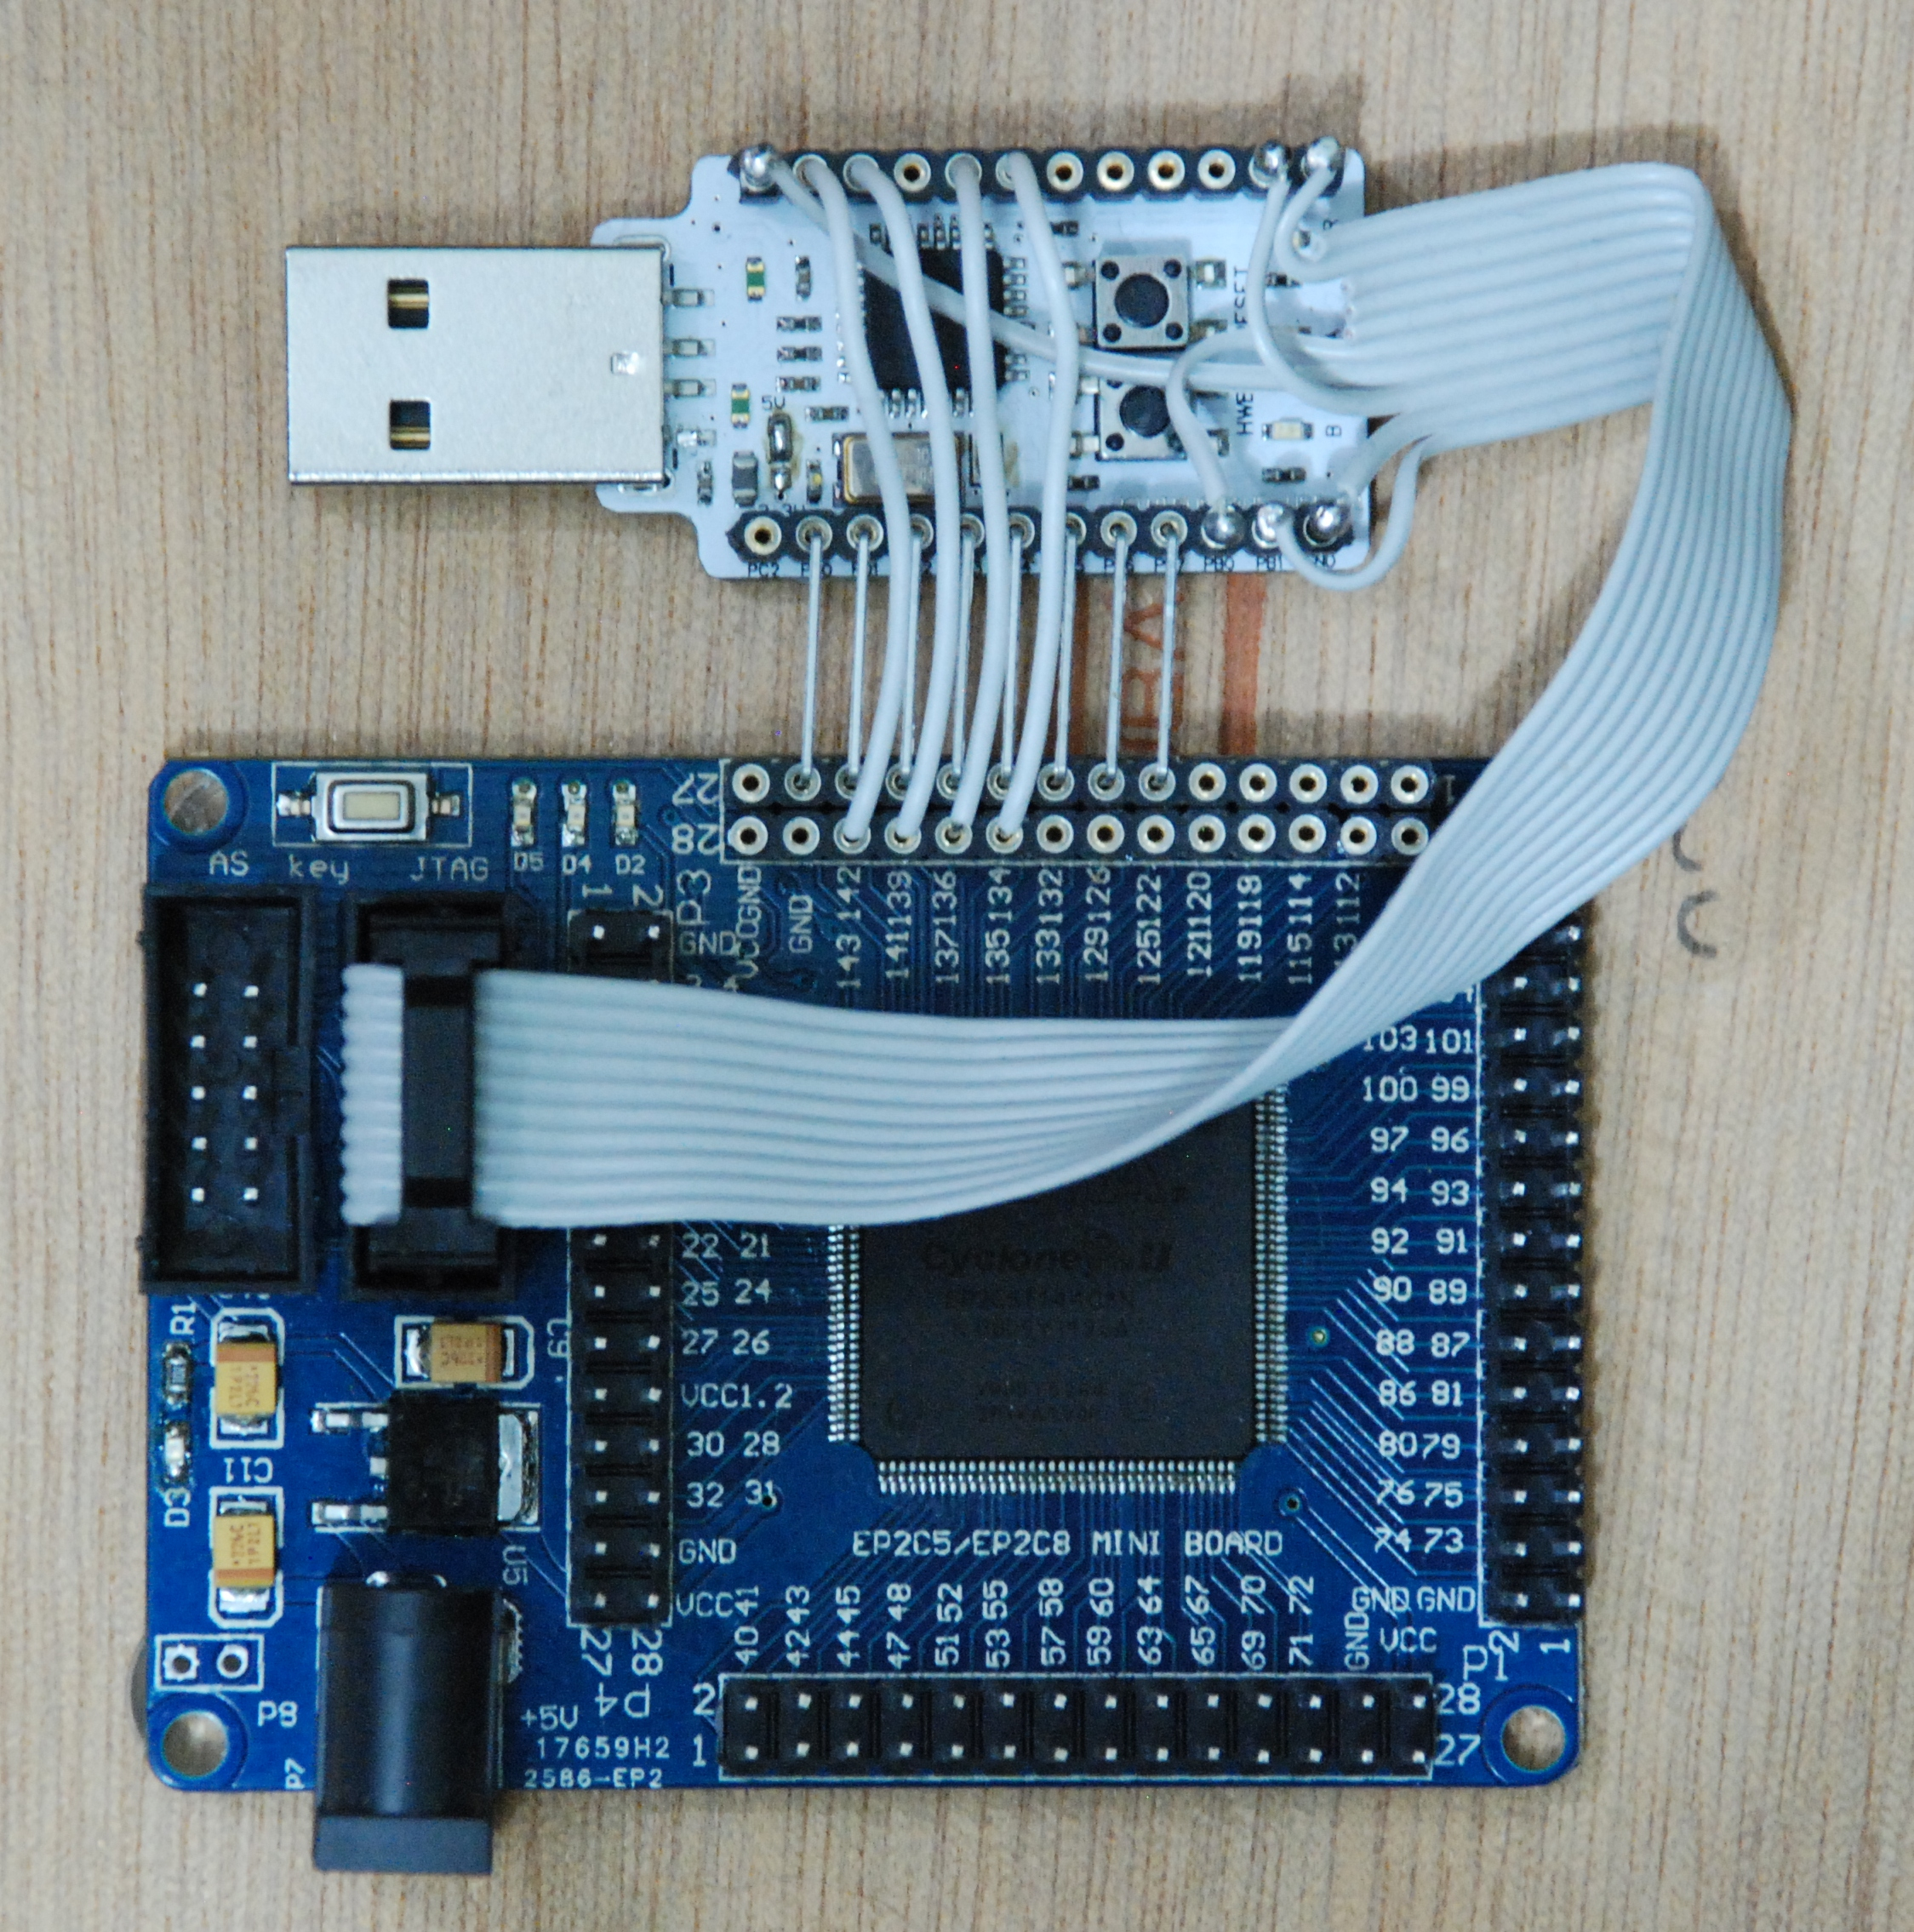
\includegraphics[width=300pt]{images/ep2c5}}

To make one you will need an EP2C5 Mini Board and a Minimus AVR USB board. The only modification necessary is to the Minimus board to allow it to draw power from the EP2C5 board. To do this you must sever the USB +5V line, which is the fourth one down on the USB connector in the picture above. Since the Minimus's connector is a Type A plug, the result is physically quite awkward if you don't have a Type A extension cable. Another option is to remove the plug altogether and replace it with a cable with a Type A plug on one end and the other end soldered to the Minimus. Thus, it becomes straightforward to connect the USB +5V power to the P8 connector in the bottom left of the EP2C5 board, to make the whole thing draw its power from USB, eliminating the need for an external +5V supply.

\subsection{Minimus/Nexys2}
Although the Digilent Nexys2 has a built-in FX2LP USB interface, in some circumstances it might be necessary to have two channels into the FPGA, either both to the same PC, or to different PCs. Here's how to wire a Minimus AVR USB board to a couple of the expansion ports of a Nexys2:

\vspace*{0.5cm}
\centerline{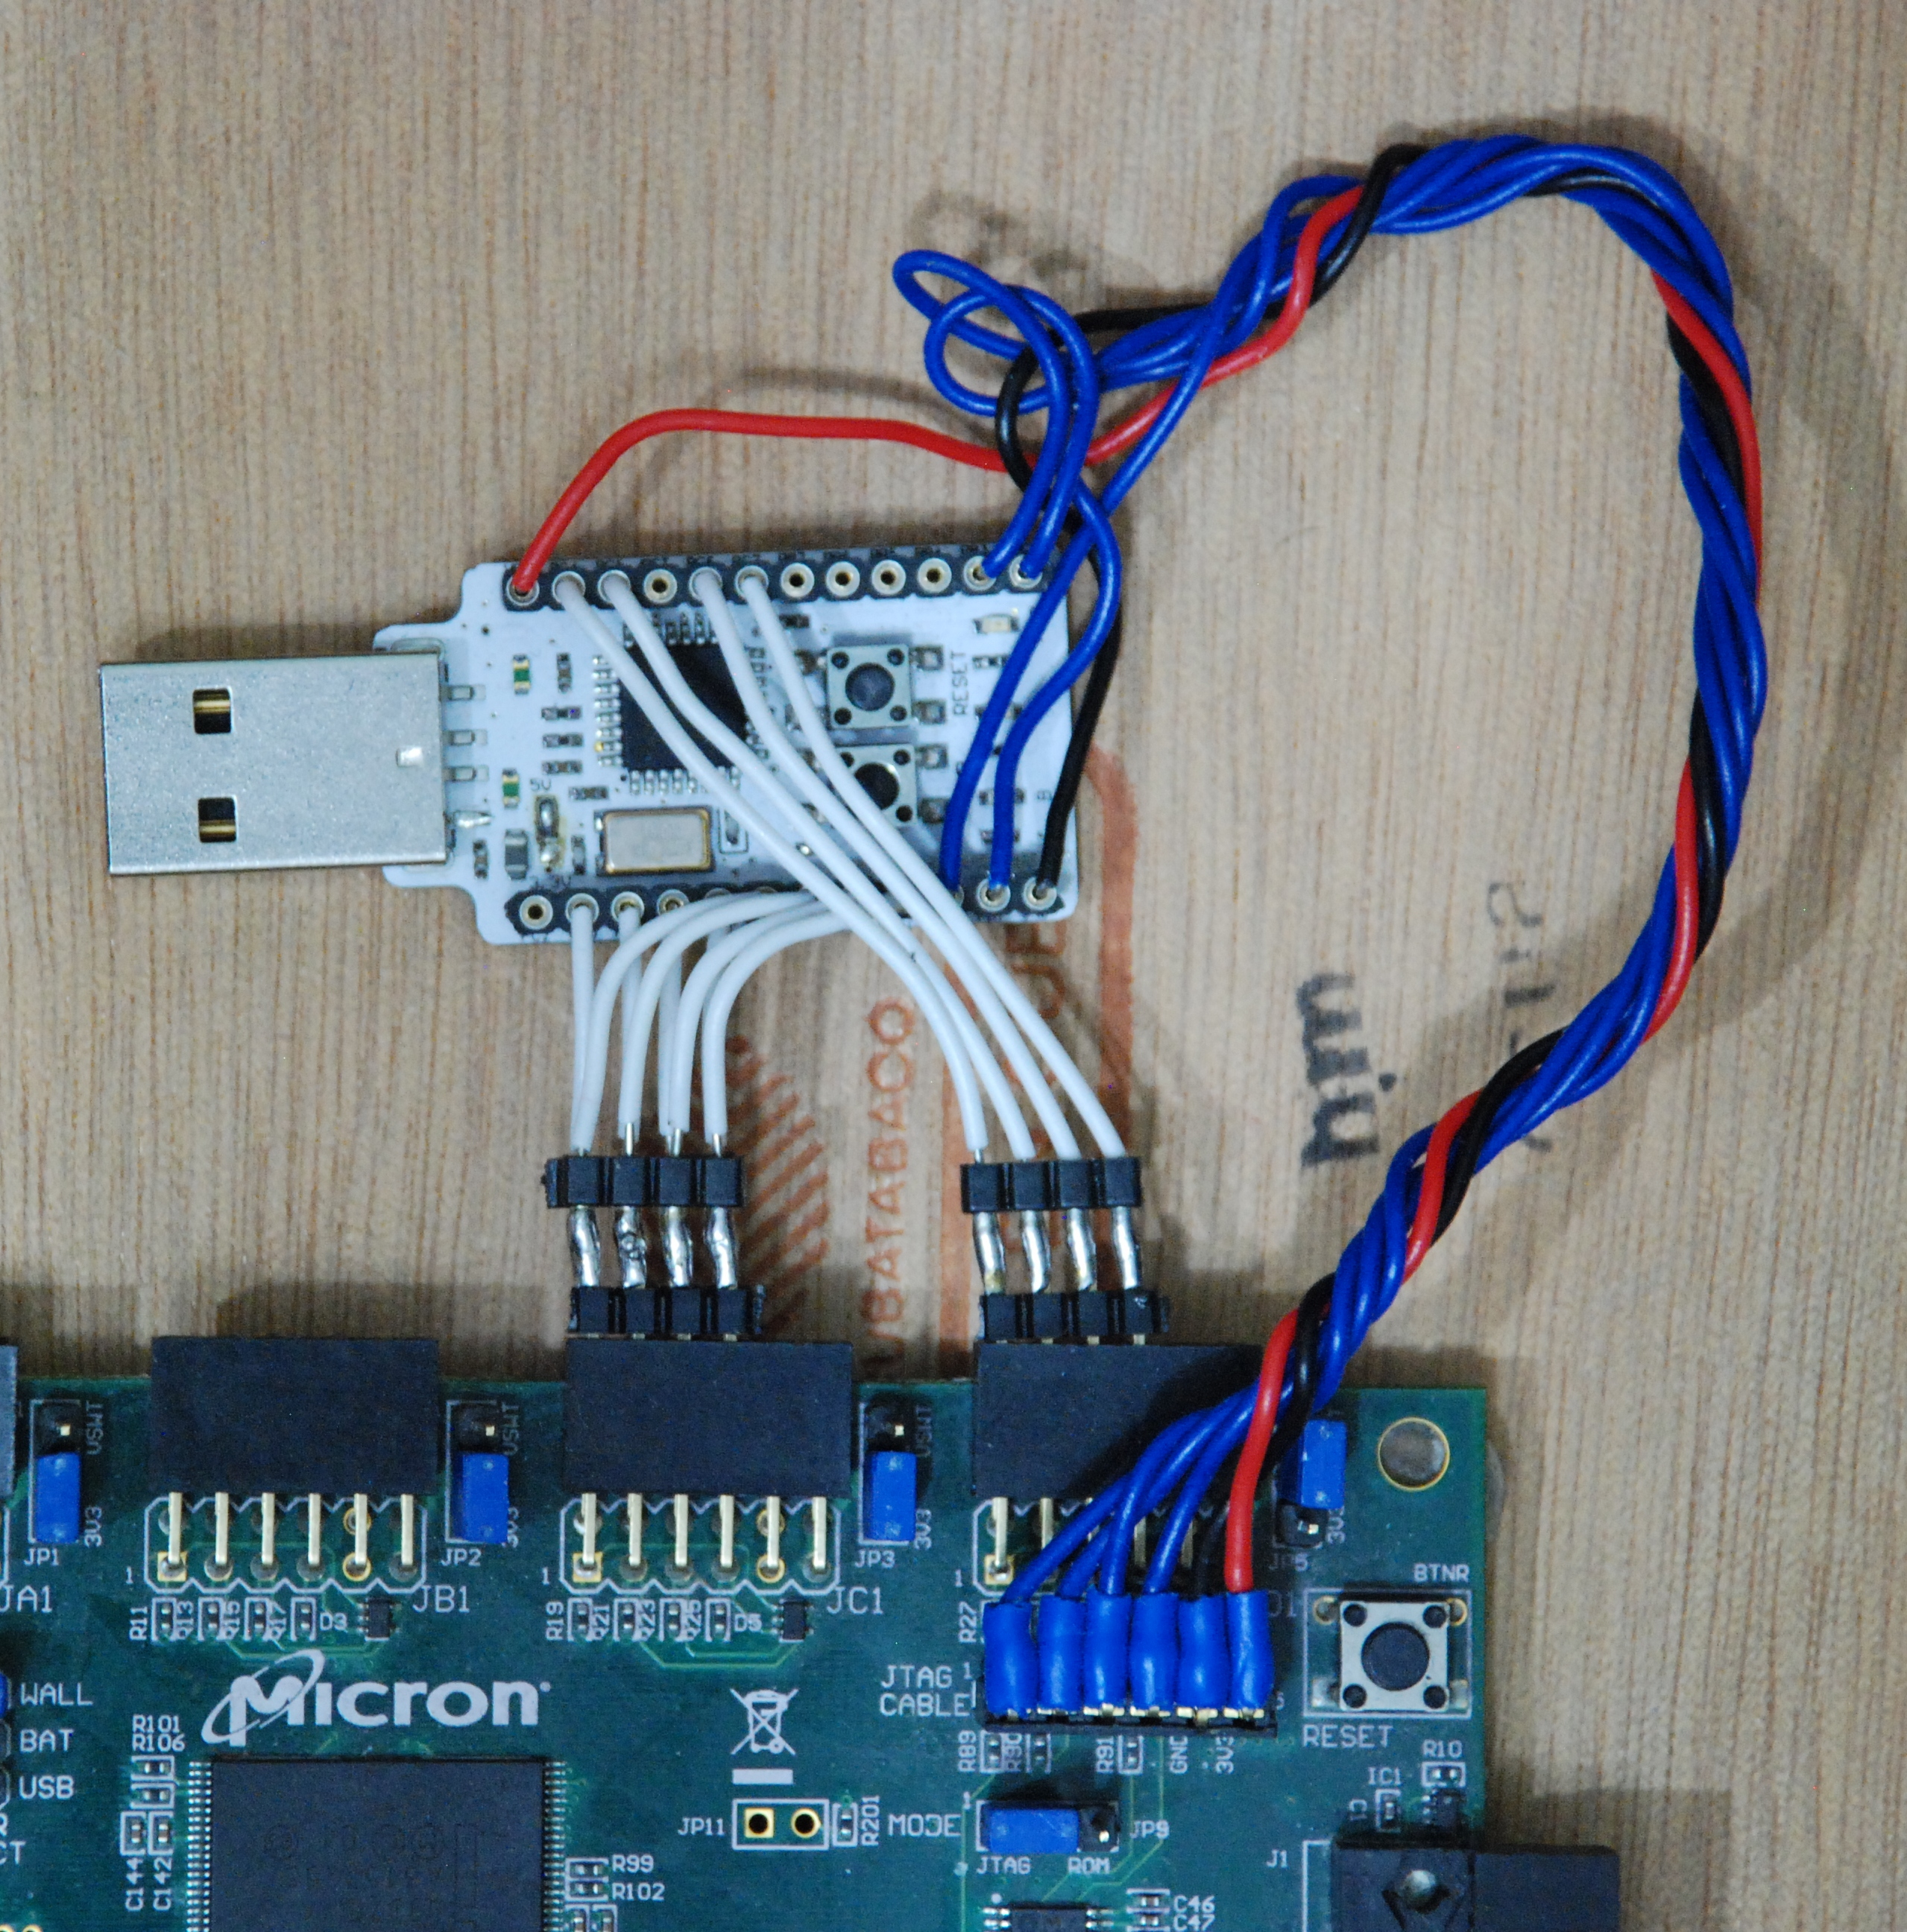
\includegraphics[width=300pt]{images/nexys2}}

The JTAG connections are \texttt{TMS} to \texttt{PB0}, \texttt{TCK} to \texttt{PB1}, \texttt{TDI} to \texttt{PB2} and \texttt{TDO} to \texttt{PB3}. The CommFPGA connections should be fairly clear from the photo: the eight data lines go from the Minimus's Port D to the top and bottom rows of the Nexys2's JC1 connector, and the four control lines go to the top row of JD1. As before, the Minimus needs to draw power from the Nexys2, so you will need to sever the USB +5V line, which is the fourth one down on the USB connector in the picture above.

\end{document}
